\subsubsection*{Tiefe aus der Pointcloud Projektion}

Wie im Kapitel \ref{sec:pc-projection} erwähnt müssen die Punkte der Project Tango Pointcloud auf die Bildebene projiziert werden und mit einer entsprechenden Tiefenfarbe und einem Radius auf den Tiefenpuffer gezeichnet werden. Dieser Schritt wurde auch bereits in Prototoypen mit den angegebenen Gleichungen umgesetzt. \\

Nach dem das Proof of Concept jedoch fertig gestellt wurde ist aufgefallen, dass OpenGL neben dem Rendering von Polygonen auch primitiven wie Punkte und Linien unterstützt. Somit konnten die Punkte im finalen Prototyp einfach vor die Kamera positioniert werden und mit Hilfe der symbolischen Konstante \enquote{GL\_POINTS} anstelle von \enquote{GL\_TRIANGLES} gerendert werden. Zudem lässt sich durch einen entsprechenden Fragmentshader die Größe der Punkte anpassen. Abbildung \ref{fig:pc-demo} zeigt links die optionale gefärbte Projektion auf der Bildebene und rechts das resultierende Tiefenbild.

\begin{figure}[h]
  \centering
	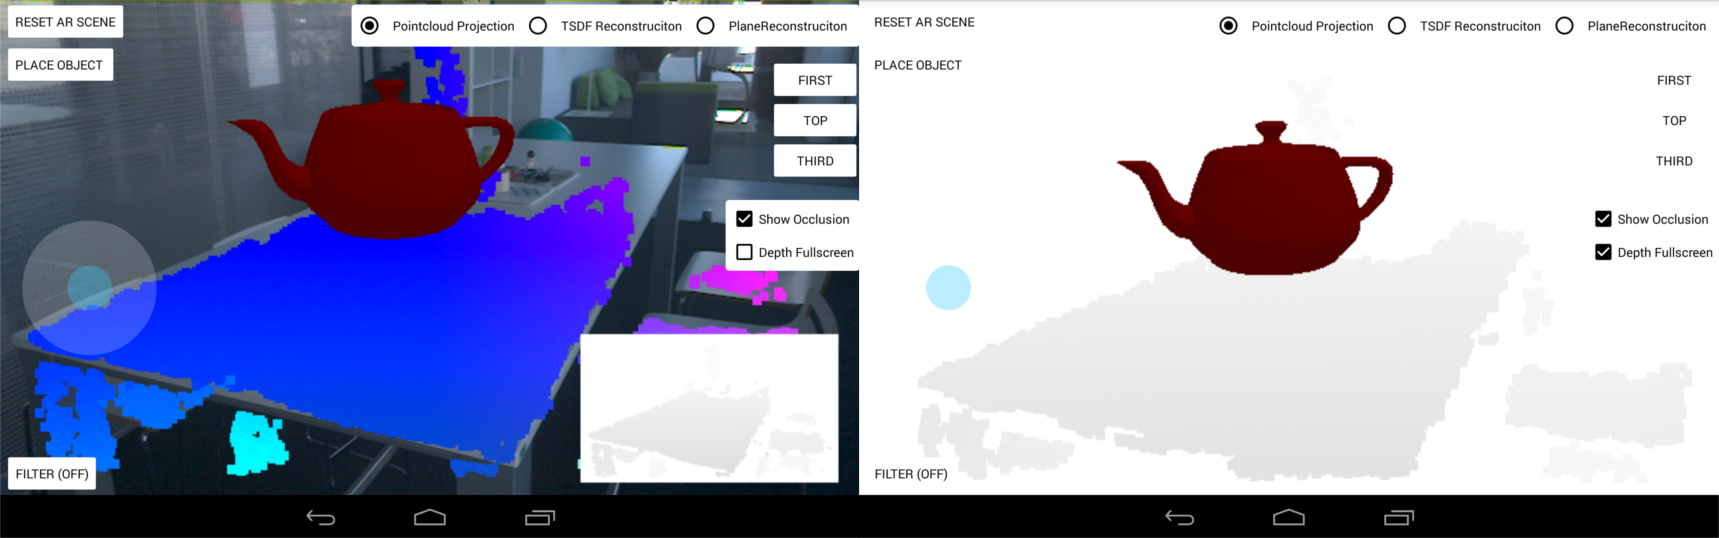
\includegraphics[width=1.0\textwidth]{content/images/implementation/pc-demo.png} 
  \caption{Pointcloud Projektion Prototyp. Links optionale Projektion auf der Bildebene. Rechts das resultierende Tiefenbild.}
  \label{fig:pc-demo}
\end{figure}




